%AFM methodology development.

%glossary nomenclature

%Have done
%Experimental setup
%AFM overview
%Script mechanics

%Todo
%Tidy MFP overview - Done
%Update Debye graph with new version - Done
%JPK overview and experimental setup - Done?
%JPK Script mechanics - Done
%Use example graphs to plot the narrative though a single example case for bin size

\chapter{Atomic force spectroscopy analysis}

\section{Introduction}

This chapter explains the experimental methods used for force curve collection as well as the computational methods used to interpret them. Over the course of data collection the process was refined to a repeatable method across a consistent experimental setup. While two different AFMs were used across the analysis, encouraged by technical limitations, they were used in such a way to complement one another. Both of these AFMs were used to produce force curves, and were interpreted using the same scripts.

\section{MFP-1D} %possibly put this first 

\begin{figure}[h!]     
        \begin{center}
          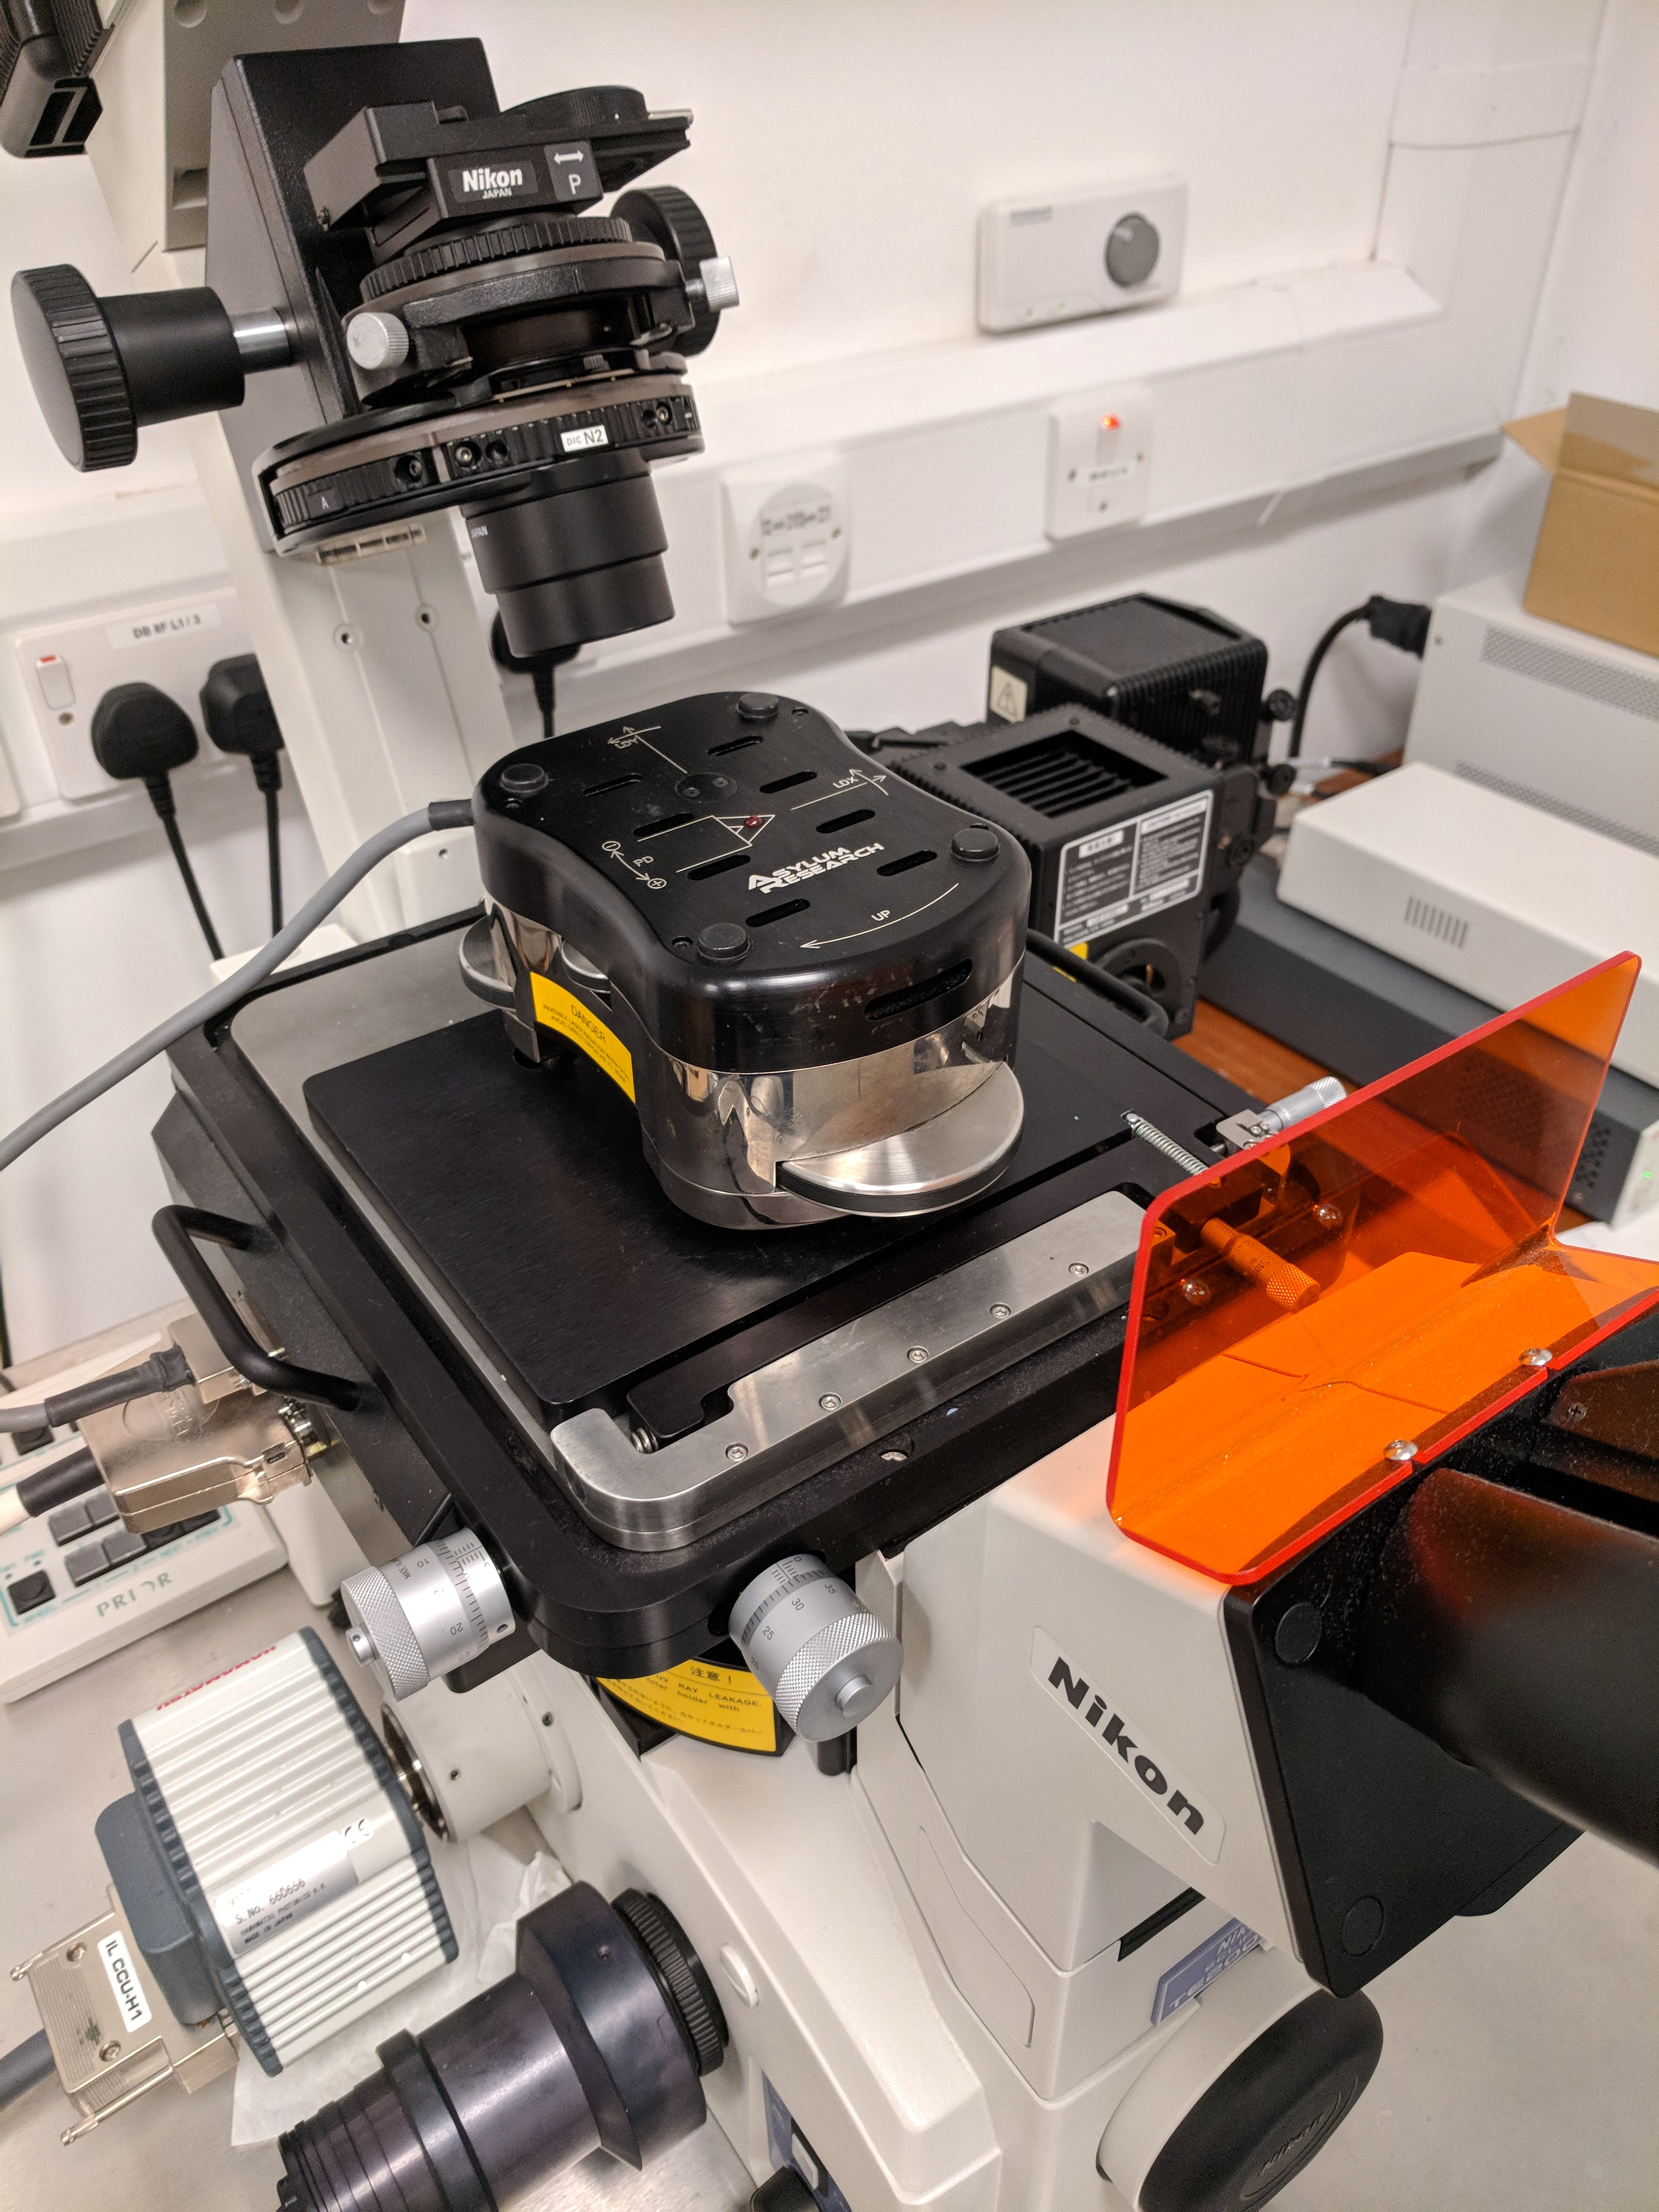
\includegraphics[width=80mm]{chapter2/forceAFM.jpg}
\end{center}
\caption{Operation setup for the MFP-1D AFM that was used for force measurements.}
\label{fig:forceAFM.jpg}                 
\end{figure}

For the force spectroscopy setup a MFP-1D from Asylum Research was used. The MFP-1D is an AFM mounted on top of an inverted light microscope, with the sample placed between the scanning head and the stage of the light microscope. In the AFM head the cantilever is mounted using tweezers in a holding apparatus. This head is immobile in the X,Y direction, horizontal movement is instead controlled by manlipulation of the stage. In the Z direction there are two possible movements - the 3 legs of the head can be moved vertically using the wheels for coarse movement, either to bring the tip in contact with the sample, or to level the head so the contact of the tip with the surface is uniform. The other control over the vertical height is via the piezoelectric transducer (piezo) mounted in the center of the head. This piezo has a travel range of roughly \SI{15}{\micro\metre}. A laser is then emitted from inside the head and directed onto the cantlever, towards the sample. (See fig ~\ref{fig:Head.jpg})

For laser alignment on the AFM head an inverted microscope is used. First the cantilever is brought into focus under the microscope, then the position of the laser is aligned atop of the intended cantilever. Afterwards the laser is focused upon the center of the tip using the sum output given by the photosensitive diode. The diode converts incident light into an output voltage, this allows the position of the laser focal point to be determined with respect to the diode boundaries.  Finally the deflection of the laser is set to 0; a central position between the positive and negative extremes. Deviation of the laser's focal point from the center point of the photodiode allows movements of the cantilever to be detected. This detects any bending (and thus attraction/repulsion) of the cantilever. 

In terms of the structure of the device, it differs slightly to the imaging AFM explained in the previous chapter; the components are more tightly packed, mounted atop of the z-piezo directly, which then brings the apparatus down onto the sample, unlike the z-piezo raising the sample up to be imaged. In addition a linear variable differential transformer (LVDT) sensor is mounted inside of the head to correct the movement of the z-piezo (closed-loop piezo) thus improving z-piezo accuracy (See fig \ref{fig:Head.jpg}).

\begin{figure}[h!]     %Insert a figure as soon as possible
        \begin{center}
          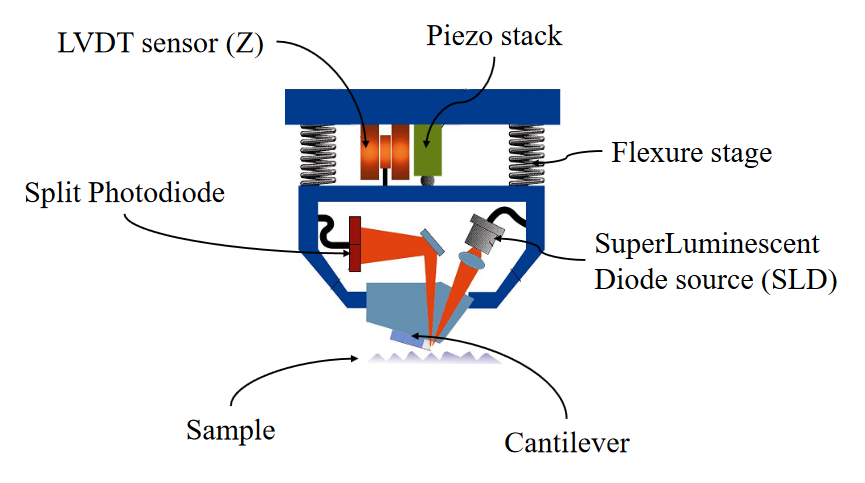
\includegraphics[width=80mm]{chapter2/Head.PNG}
\end{center}
\caption{Operational setup for the MFP-1D AFM that was used for force measurements. Adapted from \cite{AFMTalk}} %remake in jost style to reduce concerns
\label{fig:Head.jpg}                 % Reference label to the figure.
\end{figure}

%Add how vibrations in the building resolve into experimental noise and therefore dupe the system into thinking it's hit the surface.

Due to this feedback loop from the LVDT relying on previous data to define the voltage control from the next approach, the peak force (the intended maximum force applied on the cantilever per curve) was set to a relatively low number 8 nN. This was done to limit the amount of tip damage during operation. In cases where the tip fails to engage with the surface in the previous approach, this low peak force ensured re-engagement of the tip with the surface in the current loop was as gentle as possible. Noise in the data was attributable to the effect of vibrations on the operation of the instrument. When errant vibrations reach the AFM, this energy is transferred through to the cantilever, which then causes it to oscillate. This oscillation usually presents itself as a sudden spike in deflection on the curve. It is these sorts of curves that are selected and removed from the dataset. In most cases the total amount of removed curves is minimal, usually 1 or 2 per site, with a total of 100 or more curves used for processing. While it was rare that any datasets were rejected for purely noise based reasons, there is one notable set that was repeated at a later date due to a storm causing significant, persistent errors in the data. While the AFM was mounted on an anti-vibration table, the noise observed in the machine is still present.

Additionally, the standard speed of tip movement was set to \SI{1}{\micro\metre/s} (unless otherwise stated). This was done to compromise between the total dataset recording time and reduction of strain upon the cantilever and tip.

\subsection{Experimental setup}

\begin{figure}[h!]     %Insert a figure as soon as possible
        \begin{center}
          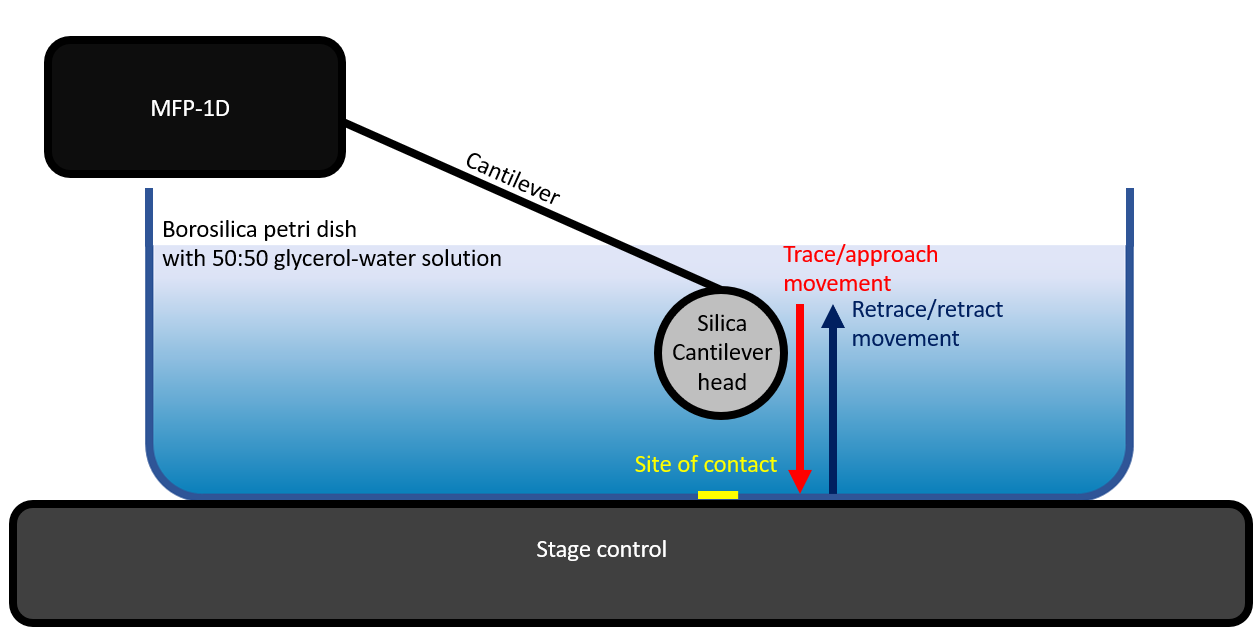
\includegraphics[width=110mm]{chapter4/Chapter4ExperiSetup2.PNG}
\end{center}
\caption{Experimental schematic of MFP-1D during operation. The AFM is abstracted away into a back box to highlight the motion that the cantilever takes with respect to the surface. The stage control provides horizontal control, and therefore moves the projected site of contact along the petri dish surface.} 
\label{fig:Chapter4ExperiSetup}                 % Reference label to the figure.
\end{figure}

%Diagram of interaction!!!!

\subsubsection{Initial Setup and Challenges}

Initially the experimental setup was focused on investigating the interactions between two silica particles. Given the difficulty in aligning two micron sized particles for interaction, the geometry of a silica particle and a flat silica surface was chosen. In order to facilitate this approach a silica particle was glued to a cantilever (see fig \ref{fig:Chapter4ExperiSetup}). These types of cantilevers are produced commercially, with the gluing process as part of the manufacturing, and were purchased to reduce experimental setup time. This cantilever was then brought into contact with a silica surface, with the results transformed using the Derjaguin approximation (See chapter 1). 

The first setup involved a \SI{1.6}{\micro\metre} diameter tip brought into contact with a silica surface glued to the inside of a plastic petri dish. This setup allowed for a liquid solution to be placed on top of the surface, contained within the plastic petri dish. A 50:50 (by volume) solution of deionised water and glycerol with a controlled concentration of LiCl was added. This ratio was chosen by volume to ensure consistent mixing and ease of preparation, given the liquid nature of both components. It was also chosen to align with Samuel C. Brown's rheological paper \cite{reference4}, which is reviewed in more detail in section 8.5.2. Glycerol was chosen for its high viscosity and low volatility, which help stabilize the solution during AFM measurements by reducing evaporation and maintaining a consistent environment for the silica particles. The increased viscosity allows for more controlled measurements of the forces between particles, providing insights into how these forces scale from single-particle interactions to multi-particle interactions within a viscous medium. This solution was brought up to completely cover the tip, ensuring the head of the AFM was submerged.

The initial setup involved calibrating the cantilever tip on a separate calibration surface (see chapter 2), then removing this surface and replacing it with the experimental one. Initially approaching the glass surface in air was of little issue, but the greatest difficulty arose in finding contact with the glass surface under liquid. Given that the liquid in use was of similar optical density to glass, the interface between the two was no longer visible under the microscope. As a result; the initial approach was slow, methodical and careful, as recklessness would break the tip. 

\subsubsection{Issues Identified and Interim Solutions}

Problems with the setup were identified after a test run, after a sweep of 4 different concentrations it was found that the resulting Debye lengths for all the curves were above 6 nm. These were directly contrary to the expectation that Debye length should decrease to theoretically 0 at increasing salt concentrations. The anomalous readings were considered to be the result of unidentified contaminants. Given the setup with the AFM was open by necessity as well as the difficulty in getting the sample under the tip in an expedient manner, there was little protection against airborne contaminants. Additionally, contaminants originating from the the plastic of the petri dish and glue were identified as a source of problems. The method of cleaning the surface was also called into question. %considering rewriting for flow
%EXPECT A VIVA QUESTION HERE!

In order to address these issues, a few changes were implemented over a series of experiments. The surface used was exposed to an improved washing protocol. This washing protocol used deionised water to clean the surface over a greater period of time. Ethanol was considered, but due to the glue holding the surface down, there were concerns over the surface having a stable platform. Additionally the method of approach was revised slightly, with a large part of the distance between the surface and the tip performed in air, with the liquid solution injected using a glass pipette slowly. This injection relied on the surface tension of the water to slowly fill the dish, resulting in a slightly higher volume use. This was done to minimize any dramatic flow from damaging the tip, emulating a normal approach submerging mechanics. %Finally any glass wear use was limited to one use only instead of attempting to clean. - I mean that's kind of standard in anything, worth mentioning?
%VIVA QUESTION POTENTIAL

Contamination issues were still present after these revisions. In order to maximise contaminant removal, the plastic petri dish was replaced with a borosilicate glass one. Instead of gluing a surface on top of the petri dish, the surface of the dish itself became the sampled area. While there had been previous considerations of the stability of the glue influencing the resulting force curve, the approach had been focused on solving the contaminant problem first. By using the surface of the dish itself, any concerns regarding glue induced artifacts could be laid to rest. This new dish permitted the use of ethanol in the cleaning procedure, as well as plasma treatment of the surface. The silica bead diameter on the cantilever was also increased to \SI{6.6}{\micro\metre} to increase the area of contact. 

Plasma cleaning was performed under a vacuum within a sealed chamber. After the chamber was evacuated a low quantity of pure oxygen gas is flowed across the surface at 0.4 bar, with the vacuum pump still active. This plasma cleaning technique cleans off any residual organic matter, resulting in water and carbon dioxide by-products. These byproducts are pumped away by the constant vacuum. \cite{PlasUV} \cite{PlasTreat} \cite{SilicaAFMCleaning}

%At this point the strong electric fields rip electrons out from the oxygen gas, forming plasma in the surrounding area. This plasma then lets off ultraviolet light, which breaks the organic bonds present on any surface contaminants. Additionally the energetic oxygen species bind to these broken bonds, resulting in water and carbon dioxide byproducts. These byproducts are pumped away by the constant vacuum. \cite{PlasUV} \cite{PlasTreat} \cite{SilicaAFMCleaning}
%(Actual values are in 2nd lab book, will be corrected after quarantine)
%Ensure this is correct

\subsubsection{Final Protocol}

In response to the ongoing contamination problems, a final protocol was established to ensure the integrity and reliability of the experimental results. The plastic petri dish was replaced with a borosilicate glass dish. Rather than gluing a surface on top of the petri dish, the surface of the dish itself was used as the sampled area. This change removed concerns related to glue-induced artifacts and facilitated a more thorough, efficient and effective cleaning method.

The glass petri dish and lid were cleaned with ethanol and water, then followed by plasma treatment. The plasma cleaning process was conducted under a vacuum within a sealed chamber, with a controlled flow of pure oxygen gas at 0.4 bar. This procedure  removed residual organic matter, further minimizing potential sources of contamination.

During the AFM setup and operation, the cantilever was carefully mounted into the AFM head, and the laser was aligned as precisely as possible to the center of the photodiode. The petri dish was then placed under the AFM head, and its surface was utilized to calibrate and calculate the spring constant of the cantilever. Following this, the cantilever was retracted by a known amount, and the liquid solution was pipetted in. After the liquid had settled, the laser was recentered to account for the change in optical density, and the tip was brought into contact with the utmost care,  relying on deflection readouts due to limited visibility. When contact was established, between 100 and 200 curves were collected for each site. In cases where multiple sites were sampled, the tip was slowly retracted, the dish was repositioned, and the approach phase was repeated to ensure consistency.

When transitioning between different electrolyte concentrations, to manage contaminants and maintain tip reusability, the tip was retracted, cleaned with water, and plasma-treated along with the petri dish. Each tip was plasma-treated no more than twice to prevent excessive damage done to the tip from the procedure (see fig \ref{fig:ScorchedEarth}). For fresh tips, they were used as supplied from the manufacturer. Direct imagining of the petri dish was not possible due to incompatible geometry at the time of collection. 
\begin{figure}[h!]    
        \begin{center}
          \includegraphics[width=90mm]{chapter4/ScorchedEarth.png}
\end{center}
\caption{The view of a damaged chip from sequential plasma treatment. Normally a clean chip presents an observed silver colour on the outside, but from over-treatment the surface has worn away, resulting in the presentation seen above.}
\label{fig:ScorchedEarth}                 
\end{figure}

\subsection{Connection with Rheology}

The choice of experimental setup, particularly the use of glycerol and the attention to contaminant control, is essential not only for the accuracy of force measurements but also for drawing connections to rheology. The increased viscosity of the glycerol solution simulates environments similar to those found in industrial or biological systems, where the rheological properties of colloidal suspensions significantly influence their behavior under shear forces. Understanding the transition from single-particle interaction forces to multi-particle interactions in these systems can provide valuable insights into the design and optimization of products and processes that rely on controlled rheology, such as in pharmaceuticals, food science, and materials engineering.

The results from this setup are intended to bridge the gap between microscopic forces and macroscopic rheological properties, demonstrating how the behavior of individual particles can scale up to influence the bulk properties of a suspension. This connection is vital for applying the findings of this study to real-world systems, where controlling rheology is key to achieving desired product performance.
%47.2 - glycerol
%


%Majority of the data collected to be around the inflection point -
%This was done to apply as little operational damage onto the cantilever. - Mention it again earlier, but less focus on the data output side.
%Mention the time factor - 0.5Hz 2s per curve. Earlier, with the experimental setup of the AFM
%Discuss in more detail about how the curve is taken though put it in chapter 2 !!
%fluctuations in the system cause the AFM to "lose" track of the surface and therefore increase the voltage input into the movement, over-correcting it's movement, shifting the captured area further up. After this the error correction it reduces the voltage until it stabilises.
%Hurricane Leslie ruining data due to location in the building.

\subsection{MFP-1D force-distance curves acquisition and processing}

\subsubsection{Acquisition}

A minimum of 100 force curve readings per site was taken for each measurement site, with the raw data saved in a single file. The columns alternated with the raw deflection reading for one curve, followed by the corresponding z-piezo value. The majority of readings measured both the approach and retract in one single motion, combining both these curves into one whole column. In the case where the cantilever was held at a certain location for a period of time, a new set of columns is appended, with another one starting after it begins movement again, thus fracturing the data whenever the cantilever is stationary between periods.

From this each curve was broken down into two lists of raw unprocessed data given by the machine; the piezo height and the deflection. The piezo height is the recorded height of the end of the piezo (where the cantilever is mounted on) on a scale of \SI{0}{\micro\metre} to \SI{15}{\micro\metre}. This range corresponds to the effective movement of the base of the cantilever in the z direction, and is thus variable between datasets, as contact can be anywhere within this range. For example, if the pizeo moves the cantilever down by \SI{5}{\micro\metre}, and then comes into contact with the surface at that area, the recorded value will be \SI{5}{\micro\metre}, not \SI{0}{\micro\metre}. It is worth noting that the z height controlled by the legs of the AFM is independent, and is not measured by the machine. Contact is a combination of the leg height being set by the operator manually, and the piezo coming into contact within its \SI{15}{\micro\metre} range. The cantilever deflection is the deviation in nm from the equilibrium position, which corresponds approximately to the center of the photodiode. No deflection (i.e. no force) is associated (by appropriate alignment) with the laser beam hitting the centre of the photosensitive two-segment diode (corresponding to 0 Volts). Deviation from the center arises from when the cantilever is bent in a certain direction,  reflecting laser off the top of the cantilever to drift along the photodiode's sensory range. This voltage is recorded as either a positive or negative voltage corresponding to upwards or downwards deflection due to repulsive or attractive forces, respectively.  This deflection is saved alongside the height in individual data files during operation automatically, with any derivative graphs following the same naming convention defined by the input file, with respect to the unpacked raw curves. 

In some cases the resultant curve is not typical. This can arise when the cantilever doesn't move far enough down to find the surface, or when the cantilever starts in contact with the surface at the start of the movement. While these curves were rare, they did occur during standard use of the AFM. These curves were removed during processing. These erroneous movements were usually corrected automatically by the AFM via error correction feedback for the successive curves afterwards. In some cases, due to imperfections of the control mechanism of the AFM, tremors/ vibrations in the building or other uncontrollable factors the frame of reference can shift up, resulting in an unusable curve, simply due to the lack of a data in a specific area. These fluctuations in the system cause the AFM to ``lose'' track of the surface and command an increase to the voltage sent to the piezo, over-correcting its movement, shifting the captured area further up. After this the error correction the peizo controller reduces the control voltage until it stabilises around the maximum force specified by the operator. In addition, in the case of an uncontrollable error (primarily vibration based) the noise of a specific curve can throw off the normal processing of the script. It is in these instances that these curves are identified and removed.

Using Python\cite{python}, an automated script was constructed to process the large volume of data generated by the MFP-1D AFM, given that each site generated around 100-200 approach and retract curves, and that multiple sites were used for each concentration, this produced a sizeable volume of data of around 6,000 curves which would be unmanageable without some form of automation.

%Overly fluffy
%A bit word salad-y too

%Make it less about the data
%appendix

%parameters:
%cfit_min
%cfit_max
%dfit_win
%dfit_off

%Rough script overview:
%Kc is calculated during AFM operation which is then added into the script by hand.

%Creation of output directory first, mfp.split_curves
%Then reads the csv if present, otherwise generates raw data files using
%mfp.comp_def_deriv
%mfp.proc_force_sep


%Afterwards plots the separation graphs with mfp.plot_force_sep_res
%Finally calculates contact forces with mfp.get_contact_forces

%mfp.split_curves
%Creates directories:
%force curves (master folder)
%raw force curves:
%- (force (N) / z piezo position (m)) %I.e. where the pizeo is in the range of it's movement (max 5um)
%Approach (see later)
%Retract (see later)

%(also removes velocity wave curves as there is only one taken at the start (and it's not always there for random reasons, but probably don't mention that)

\subsubsection{Processing}

Using numpy\cite{numpy} an array was created from the data present in the raw data file for a specific site. Each of the curves for a given site was then split up into individual numpy arrays in preparation for the following functions. As it stands, this raw data requires at the bare minimum translation from a deflection vs distance graph into a force vs distance graph. This corresponding graph of force (nN) vs z-piezo position ($\mu$m) was produced. The raw deflection was converted into force using the spring constant of the cantilever with the following equation:\cite{KcConst}. %find citation
%VIVA QUESTION - NUMPY

\begin{equation}
F = K_c(\delta - \delta _{offset})
\end{equation}

Where \textit{F} is force, $K_c$ is the spring constant, $\delta$ is the deflection and $\delta _{offset}$ is the deviation intrinsic to the cantilever under no force (taken from the start of the curve). %Unnecessary?

Similarly the z-piezo position is converted into micrometers from meters (See fig \ref{fig:EgRawGraph}). This produces an individual data file for each curve. From these curve several fitting runs were performed on this unpacked dataset to hone down the script's operational parameters (ensuring areas defined as contact and non-contact were as accurate as possible).

\begin{figure}[h!]     %Insert a figure as soon as possible
        \begin{center}
          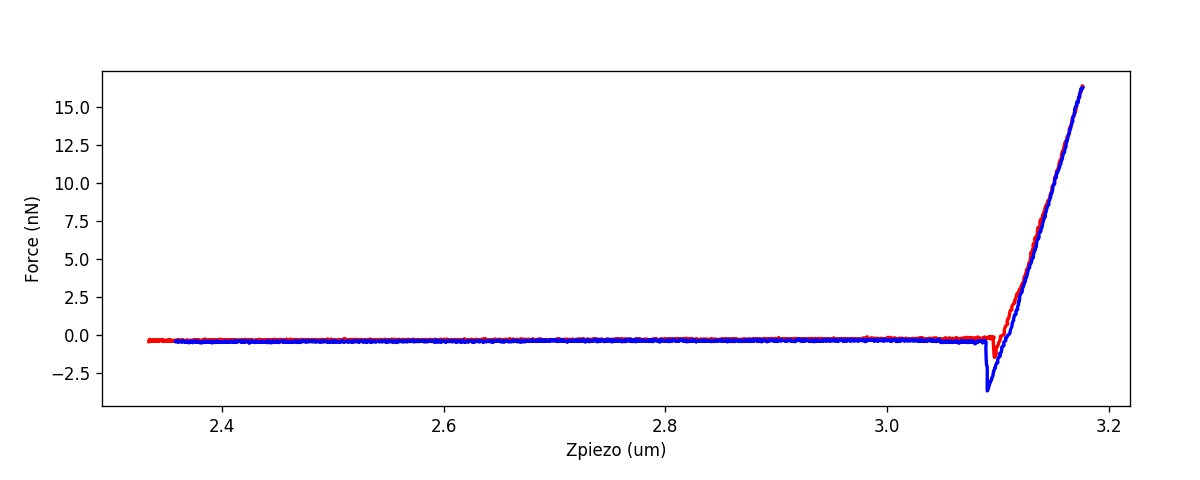
\includegraphics[width=110mm]{chapter4/EgRawGraph.jpg}
\end{center}
\caption{An example of a individual graph produced at this point. Minimal processing has been done with only the deflection converted into force (nN) vs piezo z position ($\mu$m)}
\label{fig:EgRawGraph}                 % Reference label to the figure.
\end{figure}


%Discuss how the 

In order for the script to perform correctly on each of the curves, there needs to be a long enough stretch of data for the approach and a long enough contact region. In the vast majority of cases this is true; there are a few cases where during normal operation an over correction occurs, resulting in the captured range of data to be shifted. For a given curve there are 3 identifiable regions; the approach phase, with no identifiable forces applied on the tip, the interaction phase, where the tip is either repulsed or attracted to the surface, and the contact phase, where the tip is in contact with the surface. These phases are shown in figure \ref{fig:forceAnatomy} as A, B and C respectively. A good curve will include all of these phases in it's snapshot of data, thereby allowing a clear representation of the variable forces applied upon the tip. The operational parameters of the AFM defined by the user are done so in a way to collect the most amount of data (aka setting the snapshot) during acquisition around the transitional point while reducing the amount of unneeded movement towards the surface, and equally reducing the amount of strain forced upon the cantilever during the contact region. At high strains the surface of the cantilever or petri dish can become damaged, or the cantilever can become damaged or break. As the conversion of deflection into force requires the spring constant to remain the same, and damage can cause this conversion to no longer remain true, any damage over the operation is considered by reviewing the curves over time. If there is a significant drift in the shape of the curve over the process of a site, then this is highlighted, and the experiment repeated. In the event of the cantilever breaking the AFM ceases to function and therefore data collection stops. As the retract curve immediately follows the approach curve, the retract curve inherits the same snapshot of data range.%usually followed by ample swearing

%defining the voltage input for the next step based off the previous step.

%Make frame of reference image


%Talk more about binning - find a paper

%How I know a curve is not typical by eye. Example based approach?
%Show example bad graphs

%mfp.comp_def_deriv

\begin{figure}[h!]     %Insert a figure as soon as possible
        \begin{center}
          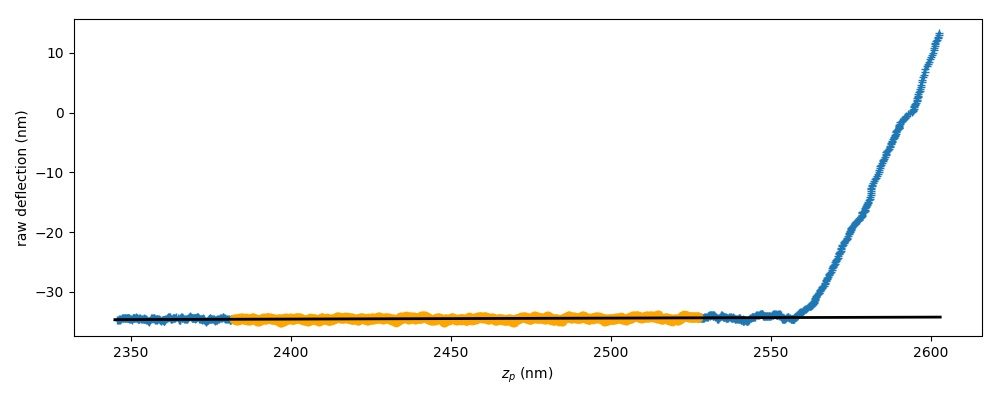
\includegraphics[width=110mm]{chapter4/farfielddrift.jpg}
\end{center}
\caption{An example of a individual graph produced for a single approach curve. The orange region of the graph is the area used in the farfield drift reduction and used to set the floor of the data to 0.}
\label{fig:farfielddrift}                 % Reference label to the figure.
\end{figure}

%proc_force_sep() and comp_def_deriv() (?)
%guess contact point and work backwards, uses np.where
%cthresh = 'first pass' guess deflection threshold for contact. cthresh is set manually
%returns de-drifted zp, df.  data used to de-drift runs from dfit_win:2*dfit_win
%remove_farfield_drift()
Each curve is then processed individually. The first step taken is to address some of the background noise. This is done by taking a linear portion of the curve (see fig \ref{fig:farfielddrift}), where any movement done by the piezo is far enough away that any forces acting between the surface and the cantilever are zero. This removes any farfield drift.  %intending to remove any gradient found along the linear non-contact region. 

This area is defined by a region along this curve, set to use points away from the initial contact area of the curve. Initially the distance traveled per datapoint is calculated by taking the adjusted range of data divided by the total number of datapoints. Based on a combination of user input and backward estimation of the contact area, the data window is carefully aligned along this linear regime. A corresponding graph is then generated to clearly highlight this selected region. This linear horizontal region is then normalised at 0, with the whole dataset translated up or down accordingly.
%Expand upon the contact area user input and estimation
%expand this paragraph

%remove_farfield_drift() end

Afterwards the data is binned into a set of variable sized bins to produce a smoother curve and reduce the effects of noise intrinsic to the system. The size of this set is determined on a case-by-case basis through an iterative process, with a bin size of 5 being most commonly used. In earlier curves where the total number of data points taken was 2000 per curve, the bin size was smaller. Subsequently the size of the data collected was larger which improved the resolution and this enhanced the data analysis. It was determined that increasing the total number of data points to 8000 was optimal. Smoothing the curve in this manner improved the accuracy in which the contact point is defined. A graph was additionally produced with a bin size sweep of $\pm$ 2 to ensure that any features were not lost during binning.
%The size of these bins were based off a paper
%describe binsize better
%Why did I pick the bin sizes that I did
%(basically binning as much data as possible to smooth the curve without losing enough data points)
%Show multiple curves to show the effect of increasing bin size? Yeh bluergh
%How do I know that changing the binsize doesn't change the result or introduce artifacts
%VIVA QUESTION

%After binning, a first degree polynomial is fitted to the selected data. In the case where a suitable fit could not be found for the curve, this set is skipped, and the curve is left untranslated.

%Review this paragraph, expand upon the "estimate produced"
Once binning was complete attention was given to the selection of the data which best represented the area in which the tip has made contact with the surface, i.e. where any piezo movement was translated into cantilever deflection. In general, this selection was defined by reviewing the graphical output from the previous steps. This selection aims to include as much as the graph as possible after the contact point, though it should be highlighted that the deflection is not a purely linear event in practice. In order to ensure that the contact region was estimated reliably, the upper and lower boundaries of the range were sweeped by $\pm$ 5 arbitrary units producing an additional series of curves with this range. This ensured that the final estimated force at contact is within a local parameter minima, i.e. the estimated contact force wasn't independently produced because of a sole artifact, but agreed with the contact forces reported from similar input values.
%Purely linear event - viva question

%Test figure to see if it's readable output in paper
\begin{figure}[h!]    
        \begin{center}
          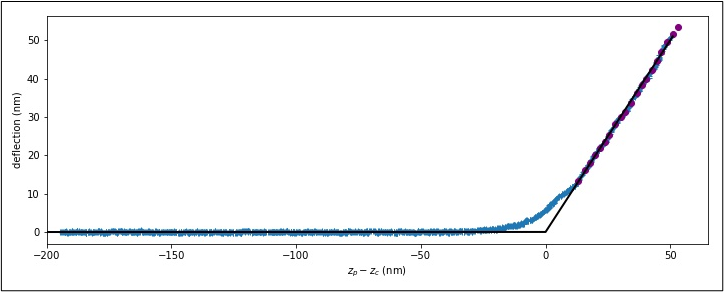
\includegraphics[width=110mm]{chapter4/contactRegion.png}
\end{center}
\caption{An example plot of an approach curve. The area used to help define contact is highlighted by the purple dots overlaying the raw curve.} %word salad
\label{fig:contactRegion}                
\end{figure}

%Put an eqn instead of word salad. Explain intercept better
%Where the extrapolation intercepts the floor line is where we define the contact point
Using this defined region, the data is extrapolated back to the intercept with the horizontal 0 force line. In the case that there is a jump to contact, the jump point is used instead of the interpolated $z_c$. Where the extrapolation intercepts the normalized floor line (i.e. where y = 0) is where $z_c$ is defined. Each curve is then normalised to 0 using z-piezo position ($z_p$) minus z-piezo contact point ($z_p$ - $z_c$) at the point of contact (see fig \ref{fig:contactRegion}). This term is defined as z-separation ($z_\text{sep}$). By defining the contact point as 0 the force at contact can be extrapolated from the curve - by taking the equivalent y-axis value when x is 0.

In some cases, particularly in the measurements made with the JPK NanoWizard AFM (see Section 8.3), intermediate data points through the jump to contact were successfully captured, providing further insights into this phase of the force profile. These data points offer a more detailed understanding of the transition and are discussed in greater depth later in the thesis.

\begin{equation}
z_\text{sep} = z_p - z_c
\end{equation}

%TODO add graph showing a jump to contact calculation

In conceptual terms $z_{sep} \textit{= 0}$ is the point in which the cantilever would come into contact with the surface under no outside stress. In some cases, when a high degree of cantilever movement is applied in the contact phase, the cantilever can bend beyond the the non-linear region of the photodiode detector. This is only present at high deflections, and thus care is taken to ensure that the analysis is done within the linear response region of the photodiode. The non-linear region is where the laser reaches the limits of the photovoltaic cells and the overall signal strength is reduced. Additionally, at higher stresses the cantilever can be subjected to non linear deformation. As the system itself assumes a constant translation from piezo movement during the contact phase into linear deflection recorded by the photodiode, these abnormal data points at the end of the curve are a result of the photodiode's limits. It is in this cases that said recorded can interfere with the processing. as a result, where the behaviour of the curve is inconsistent with the known behaviour of the machine, that said data is removed, though it is important to highlight that said abnormal data only appears after an expected linear contact phase, when the limits of the machine are met. This curve then displayed expected behaviour throughout the approach, interaction and contact phases.

Later in the thesis, particularly in Section 7.5, measurements made with the JPK NanoWizard AFM reveal additional aspects of this part of the force profile, including the "jump to contact" phenomenon. These subsequent findings provide a more nuanced understanding of the force interactions and should be considered alongside the  observations presented here for a more complete picture.
%VIVA QUESTION

After all this processing an averaged curve is is generated by taking all of the individual curves and averaging them together. This is done by progressing along the $z_{sep}$ list, combining their points into a binned point, averaging each bin, then calculating the standard deviation of each bin.

\begin{figure}[h!!!!]    
        \begin{center}
          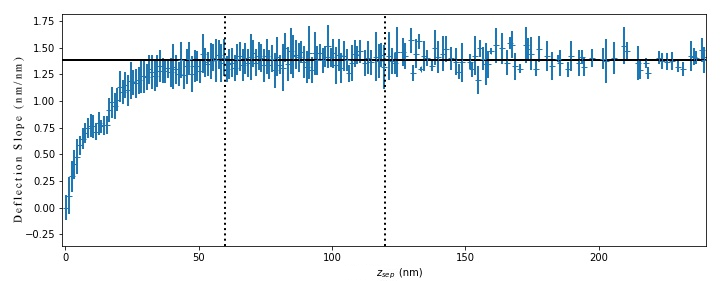
\includegraphics[width=100mm]{chapter4/gradientGraph.png}
\end{center}
\caption{An example plot of the averaged approach gradient. The "approach gradient" in this context refers to the slope of the deflection as the AFM tip approaches the surface. Specifically, it is the rate at which the deflection changes as the AFM piezoelectric element moves the cantilever closer to the sample surface. This gradient provides insight into the force interactions occurring as the tip nears the surface, which is critical for understanding phenomena like the "jump to contact." This graph focuses specifically on the region after contact and the area used to define contact is highlighted by vertical dotted black lines (aka the defined contact region). The horizontal black line indicates the extrapolation of the data. in this case the data is binned to reduce noise. The height of each blue bar indicates the standard deviation for each point.} %units, better y axis
\label{fig:EgAvgDeriv}                
\end{figure}

%Add equation
In order to ensure that the region defined by the operator is correct, a number of diagnostic graphs were produced in order to aid the selection process. The gradient of the deflection is calculated with respect to the stage height in order to highlight the transition between the movement phase and the contact phase of the graph. This is done for individual curves as well as an averaged curve (see \ref{fig:EgAvgDeriv}).

\newpage

These curves are then all plotted on top of one another to check that all curves follow the same rough shape (see fig \ref{fig:proc_force_sep_mastercurve}).

\begin{figure}[h!]     %Insert a figure as soon as possible
        \begin{center}
          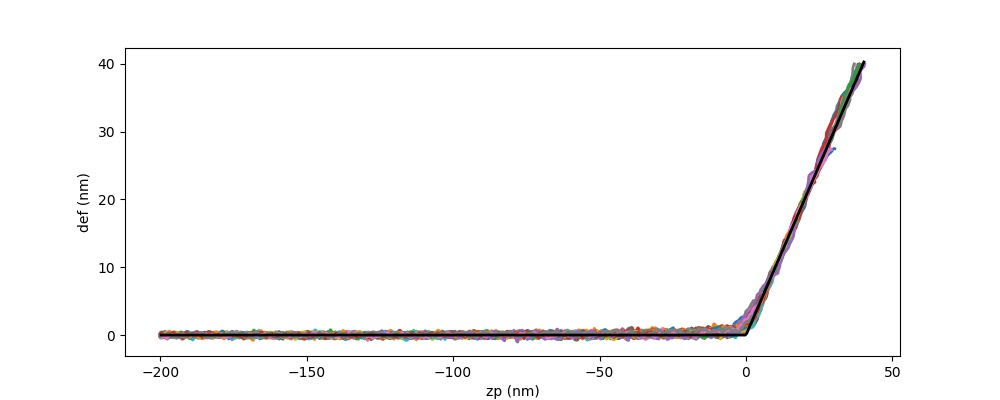
\includegraphics[width=110mm]{chapter4/proc_force_sep_mastercurve.jpg}
\end{center}
\caption{An example plot of all the curves for a given site processed up until this point. A reference black line is overlaid demonstrating what a curve would look like with only terminal electrostatic repulsion. This figure represents about 100 curves aligned atop one another.}
\label{fig:proc_force_sep_mastercurve}                 % Reference label to the figure.
\end{figure}

%histogram of detection slope, not sure if it's worth mentioning, mostly a quick check to see nothing crazy happens

%#mfp.proc_force_sep END

%mfp.plot_force_sep_res 



This resolves in a final averaged and binned force curve (see fig \ref{fig:EgFinalCurve})

\begin{figure}[h!!!]     %Insert a figure as soon as possible
        \begin{center}
          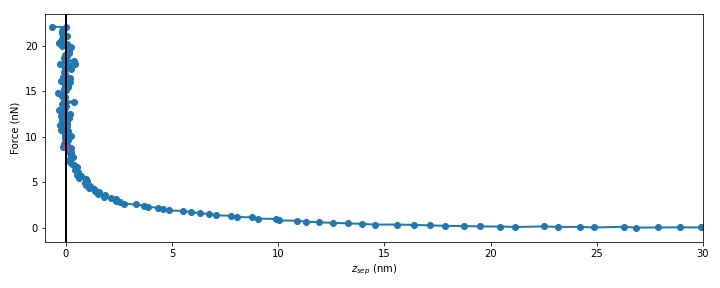
\includegraphics[width=110mm]{chapter4/EgFinalCurve.jpg}
\end{center}
\caption{An example plot of the final processed force curve. The y axis has been translated to show the distance from contact, with a black line highlighting the defined point of contact. The datapoint used to define the force at contact is highlighted in red.}
\label{fig:EgFinalCurve}                 % Reference label to the figure.
\end{figure}

%mfp.get_contact_forces

Afterwards the focus of the script changes to calculating the force applied at contact. Positive forces indicate a repulsive force, negative forces indicate an attractive force. A Savitzky--Golay filter is applied to the data to reduce the noise intrinsic to the data. \cite{SavitzkyGolay} Then the curve is followed algorithmically until it passes over the threshold point - by default, this threshold is defined as the point where the separation between the AFM tip and the surface is 0 nanometers, indicating physical contact.
%VIVA QUESTION

This is done for each individual curve, eventually resulting in a histogram of contact forces (see fig \ref{fig:EgForceHisto}). This provided an insight into the variance between each of the curves, with a wide distribution indicating improper calibration settings for some of the curves. In the cases of outliers, their individual curves were reviewed and used to improve the fitting parameters.

\begin{figure}[h!!!] 
        \begin{center}
          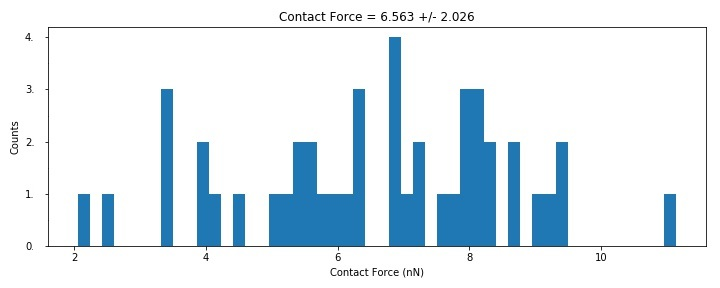
\includegraphics[width=110mm]{chapter4/EgForceHisto.jpg}
\end{center}
\caption{An example of a histogram produced from a set of curves for specific site. The mean force is given at the top with the standard deviation.}
\label{fig:EgForceHisto}              
\end{figure}
%VIVA QUESTION - statsitical properties of distribution

Contact force refers to the force exerted when the AFM tip makes physical contact with the sample surface. This force is measured at the precise moment when the separation between the AFM tip and the surface reaches zero. It can be either repulsive or attractive depending on the nature of the interaction between the tip and the sample. Positive values indicate a repulsive force, often due to surface stiffness or electrostatic repulsion, while negative values signify an attractive force, such as van der Waals forces or adhesion.

In all cases the total number of individual graphs per final force datapoint is between 80-200 curves.

\subsection{Validation of results}

In order to validate that the data produced by the procedure met the precedence set by theory, the Debye length was experimentally determined. This approximation of the Debye length ($\kappa$) was calculated using the equation outlined in chapter 1 (see eqn $1.2$). The experimentally calculated value was then checked against the approximated Debye length across a sweep of concentrations. This was in part to ensure that the procedure gave sensible results as well as a means of detecting invisible sources of contamination.

\begin{figure}[h!!]    
        \begin{center}
          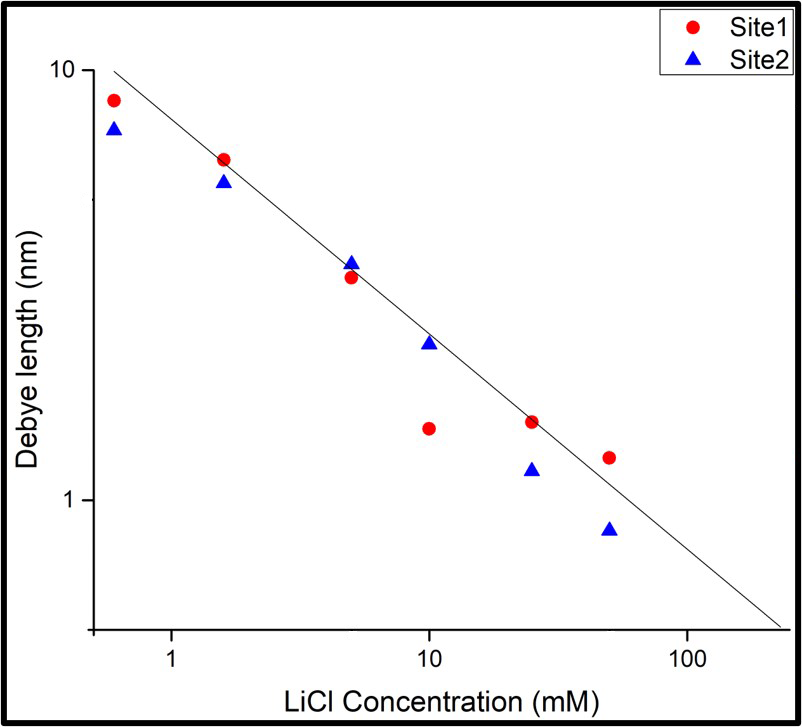
\includegraphics[width=100mm]{chapter4/DebyeLength.png}
\end{center}
\caption{A preliminary graph produced to investigate the expected Debye length vs the recorded Debye length at different salt concentrations. The black line indicates the approximated $\kappa$, whereas site one and two are two different recording areas on the glass surface.}
\label{fig:DebyeLength}                 
\end{figure}

This procedure produced sensible Debye length measurements according to the preliminary data (see fig \ref{fig:DebyeLength}). As a result this procedure was used for subsequent experiments. The Debye length of the interacting silica sphere was calculated by calculating the equation of the curve during the interaction phase and extracting the exponent component (i.e. between the approach and contact phases).
%These curves were used for analysis using the following script mechanics.

%From these results a selection of the concentrations where an observable Debye length was chosen and processed using all of the techniques outlined in this chapter. 
This Debye length measurement procedure indicates strongly that the chosen experimental and processing protocol is appropriate. Additionally the influence of contaminants have been reduced to a minimum from said revised protocol.

\newpage

\section{Nanowizard}

Over the course of the investigation the availability of an alternative AFM became available. When compared to the MFP-1D, the setup is very similar, with one notable exception. This AFM allows for free horizontal control coupled to the AFM head, instead of requiring the operator to disengage each time. Aside from the time saved between changing sites, this allows for techniques such as force mapping to be used (See chapter 2). The setup procedure remained the same as defined before during use with this AFM with any difference being software based, and thus an unnecessary detail for this report. 

\begin{figure}[h!]     
        \begin{center}
          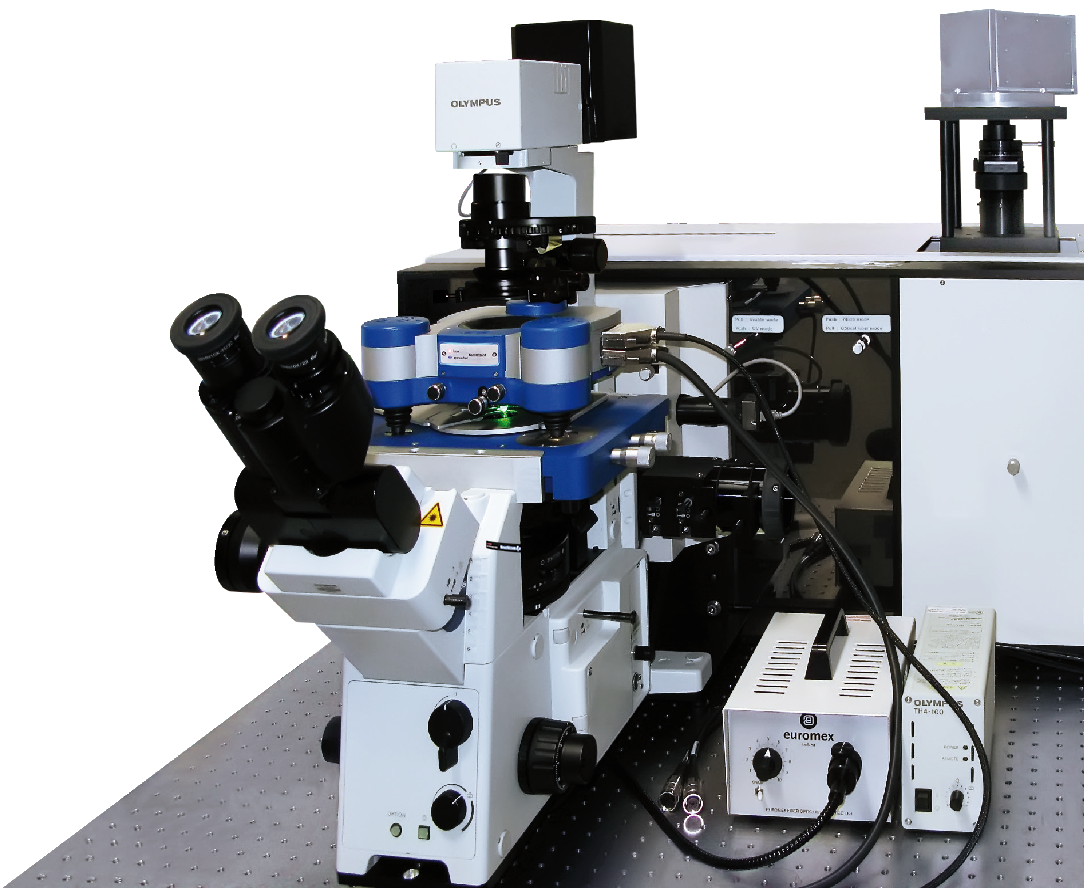
\includegraphics[width=80mm]{chapter4/Nanowizard.png}
\end{center}
\caption{Operation setup for the Nanowizard AFM that was used for force measurements \cite{NWizardPic}.}
\label{fig:Nanowizard.png}                 
\end{figure}

Fortunately the previously established sample preparation and cleaning procedure was adapted with little difficulty with the experimental throughput considerably increased. The tip speed was set to the previously defined speed, \SI{1}{\micro\metre/s} as well as the peak force at 8 nN, unless otherwise stated.

\subsection{Analysis differences for JPK NanoWizard} %What is this an RPG tabletop for scientists?

The output from the Nanowizard was exported from the proprietary JPK file format and refitted to work with the script described above. While the differences in output data structure is dramatic, this was handled by a short reformatting script to translate the data into a usable format. The only differences of note between the two is that the JPK format has fewer significant figures compared to the previous methods.

In the case of force mapping, there are considerably less curves per site. At this point, the previously established curves produced by the MFP-1D for each concentration were used for comparison. Each of the curves is then processed by the script, with a note taken of its x,y $\mu$m offset. Afterwards the averaged contact force (for approach) or adhesive force (for retract) is plotted on a heat map. For each heat map a 10$\times$10 grid was processed, with at minimum 3 curves per site taken, with a \SI{1}{\micro\metre} distance between each site. It should be noted that the software processes an entire grid first, which is to say each site is repeated after all sites of the current grid are done.

\section{Development and Significance of the Force Curve Analysis Software}

The analysis software developed during this research plays a pivotal role in the extraction and interpretation of force curves obtained via Atomic Force Microscopy (AFM). The ability to automatically process large volumes of data with high accuracy and consistency is a key contribution of this thesis, making the software not just a tool, but a significant contribution to the field.

Traditional methods of AFM data analysis often rely on manual interpretation of force curves, which can introduce variability and error due to human judgment. While earlier software tools provided some level of automation, they often lacked the flexibility to handle complex datasets or adapt to the specific needs of different experiments. Equally, the availability of the software is often tied to specific manufacturers and distributors, which limits accessibility. The software developed in this thesis builds on these earlier approaches by offering a more robust, adaptable, and user-friendly platform that can be adapted to any set of results.

This software was designed to address several key challenges. Firstly, by incorporating advanced smoothing techniques, such as the Savitzky-Golay filter, the software effectively reduces intrinsic noise while preserving critical features of the data, such as the 'shelf' observed in certain force profiles. Secondly, the variable-size binning approach allows for more precise control over data smoothing, enabling the detection of subtle force interactions that might be lost in more rigid binning protocols. Finally, the software automates curve fitting to theoretical models, reducing the need for manual intervention and ensuring that the analysis is both consistent and reproducible across different datasets.

One of the significant improvements brought by this software is its robustness against the variability inherent in AFM data. This robustness is particularly evident when comparing the software's performance with older systems that may produce noisier data. The ability to extract meaningful information from such data extends the lifespan of older AFMs, making them viable for current research without the immediate need for expensive upgrades.

The software’s robustness was validated through the analysis in this thesis, given in the following chapters. The consistency of the Debye length calculations across different concentrations, as well as the successful extraction of the 'shelf' feature in noisy data, are testaments to its reliability.

By making this software open source and accessible to the broader scientific community, this thesis not only contributes to the field of AFM but also democratizes access to high-quality data analysis tools. The flexibility of the software allows researchers to adapt it to their specific needs, potentially leading to new discoveries and innovations in surface force studies. It bridges the gap between traditional manual methods and the need for high-throughput, consistent analysis in modern AFM studies.


%TODO: INSERT HEAT MAP HERE LATER AFTER SCRIPT IS DONE BECAUSE AAARGGH

%Show example heatmap

%include any changes observed here. Only difference so far is that it's a faff and that the sig figs is lower on the JPK file format.


%%%Review later:




%%Insert graph showing selection window
%Possibly go into more detail
%Actually do
%Just not right now, your mind can't make sense of it